\tableofcontents

\clearpage
\pagenumbering{arabic} % Arabic (standard) page numbering
\chapter{Introduction}

Dans le cadre du cours de compilateur, ce projet à pour but de créer un transpilateur de code python en code \textbf{C++}.
Pour ce faire ce programme utilise une implémentation de lex et yacc en python (package \textbf{ply}~\cite{ply}).
Dans la première partie de ce rapport se trouve l'analyse de la problématique ainsi que les différentes fonctionnalités de ce programme.
Puis, dans une deuxième partie, la réalisation des différentes fonctionnalités implémentée.
Et finalement les résultats obtenus ainsi que la conclusion de ce projet.
\chapter{Analyse}

Le but de ce programme est de transformer du code \textbf{python} en \textbf{C++}.
le programme doit être capable de détecter et transformer en \textbf{C++}:
\begin{enumerate}
    \item Les variables
    \item La portée des variables
    \item Les opérations de base (+, -, *, /, <, >, \%, <=, =>, ==, !=)
    \item Les structures (while, if, elif, else)
    \item Les fonctions
\end{enumerate}

Python étant un langage indenté et non typé, le programme doit également être capable de gérer
le typage des variables et remplacer les indentations par des \textbf{\{\}}.

\chapter{Réalisation}

Lors de la réalisation du programme, nous avons séparé le programme en 3 parties :

\begin{itemize}
    \item Analyse lexicale
    \item Analyse syntaxique (cf. \hyperref[annexe:grammar]{Grammaire})
    \item transpilateur
\end{itemize}

\section{Gestion des types}
~\label{section:Type}

Les types gérés par notre programme sont:
\begin{enumerate}
    \item Float
    \item Int
    \item String
    \item Bool
\end{enumerate}

\subsection*{Analyse lexicale}

Le type de variable est détecté avec des regex pour chaque type énuméré ci-dessus.

\subsection*{Analyse syntaxique}

Lors de l'analyse syntaxique, seul le typage des fonctions est traité. (voir section \hyperref[section:Fonctions]{Gestion des fonctions}).

\subsection*{Transpiler}
Le transpiler permet de faire des opérations entre les variables de même type.
Il ne permet pas de faire des conversions implicites de type. par exemple  \(Float+Int\)

\newpage


\section{Gestion des opérateurs de base}

Les opérateurs gérés par notre programme sont:
\begin{enumerate}
    \item \(+\)
    \item \(-\)
    \item \(/\)
    \item \(<\)
    \item \(>\)
    \item \(\%\)
    \item \(<=\)
    \item \(=>\)
    \item \(==\)
    \item \(!=\)
\end{enumerate}

\subsection*{Analyse lexicale}

Lors de l'analyse lexicale, les opérateurs font partie des caractères réservés de notre programme et sont directement à détecter.

\subsection*{Analyse syntaxique}

Lors de l'analyse syntaxique, les opérateurs détectés dans lexer sont transformés en nœud selon quelles opérations est détecté.

\subsection*{Transpiler}

Lors de la transpilation, les variables déclarer avec des opérateurs booléens sont détectés est créé avec le typage \(bool\).
La gestion des types dans les opérations sont gérées comme indiqué dans la section \hyperref[section:Type]{Gestion des types}.

\section{Gestion portée des variables}

La portée des variables est similaire à celle du langage python.
Le programme détecte les variables globales et les variables locales, cependant si une variable est définie en dehors de tout bloc (fonction,boucles,conditions), lors de l'appel
de la variable dans un bloc elle sera recréée si dans le programme python le mot-clé global n'est pas précisé.

\newpage
\section{Gestion des structures (boucles,conditions)}

\subsection*{Analyse lexicale}

Lors de l'analyse lexicale, les structures font partie des mots réservés de notre programme et sont directement détectées.

Liste des mots réservés:

\begin{enumerate}
    \item while
    \item if
    \item elif
    \item else
\end{enumerate}

\subsection*{Analyse syntaxique}

Sur la figure \ref{exemple_struct} un exemple de l'arbre syntaxique des structures gérées par notre programme

\begin{figure}[h]
    \centering
    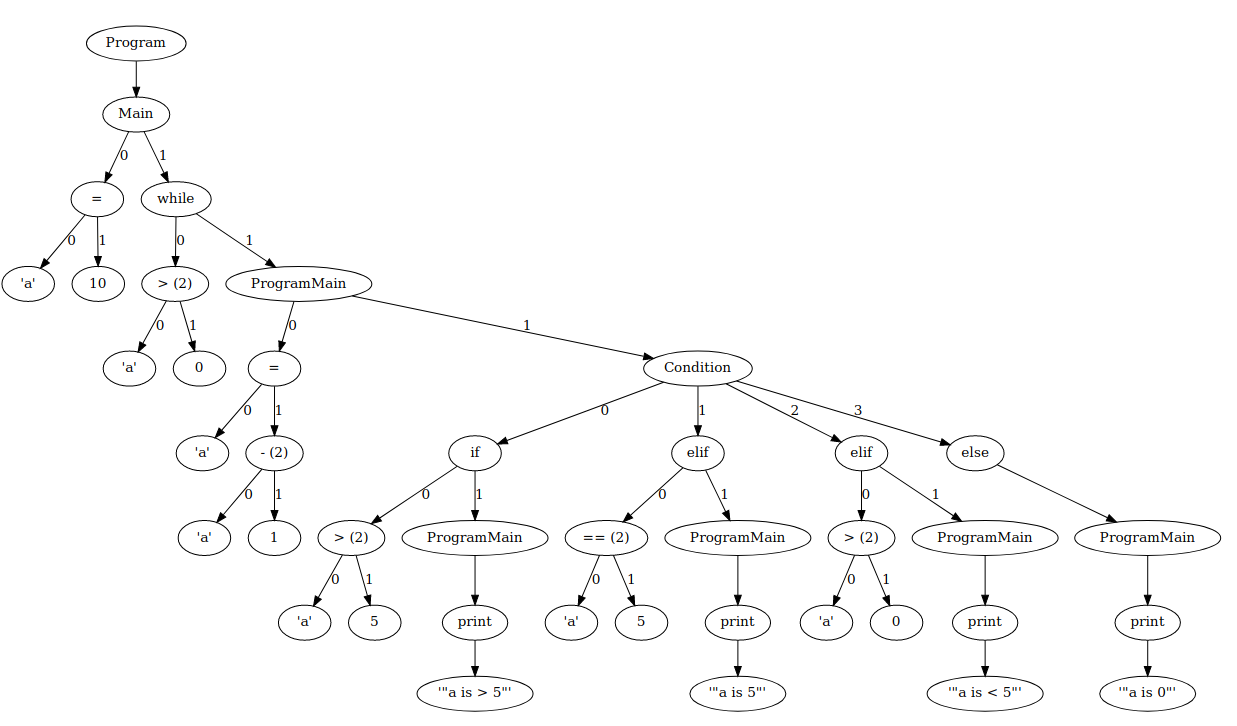
\includegraphics[width=0.8\textwidth]{./images/exemple_ast_struct.png}
    \caption{Exemple AST structures}\label{exemple_struct}
\end{figure}

\section{Gestion des fonctions}
~\label{section:Fonctions}
en \textbf{C++} le programme principal ce trouve dans une fonction main et à l'intérieur de celle-ci on ne peut pas créer d'autres fonctions.
Pour recréer ce comportement nous avons décidé de brider notre code python en l'empêchant de créer des fonctions
à l'intérieur d'un bloc \verb|if __name__ == "__main__"| qui nous sert de fonction main.
\newline
\newline
Il est également important de noter que les fonctions gérées par notre programme doivent être typées comme sur l'exemple ci-dessous:
\lstset{language=Python}
\begin{lstlisting}
    def fo(x:int) -> int: # fonction prenant un entier et retournant un entier
    def fo2() -> None: # fonction de type void
    \end{lstlisting}


\subsection*{Analyse lexicale}

Lors de l'analyse lexicale, les fonctions sont détectées avec le mot-clé \textbf{def} alors que la fonction \textbf{main} est
détectée avec un regex.

\subsection*{Analyse syntaxique}

Lors de l'analyse syntaxique, le programme distingue 2 types de déclaration de fonctions, la première a des arguments et la deuxième non.
Dans les 2 cas, le nœud d'une fonction va contenir le type de retour et le programme dans la fonction.
Mais si la fonction possède des arguments, ils doivent alors également être traités et ajouter au nœud.

Pour l'appel de fonction on retrouve nos 2 types comme pour la déclaration, un avec paramètre et un sans.
Comme précédemment dans le cas où l'appel contient des paramètres, un nœud de paramètre doit être ajouté à la fonction.


\begin{figure}[h]
    \centering
    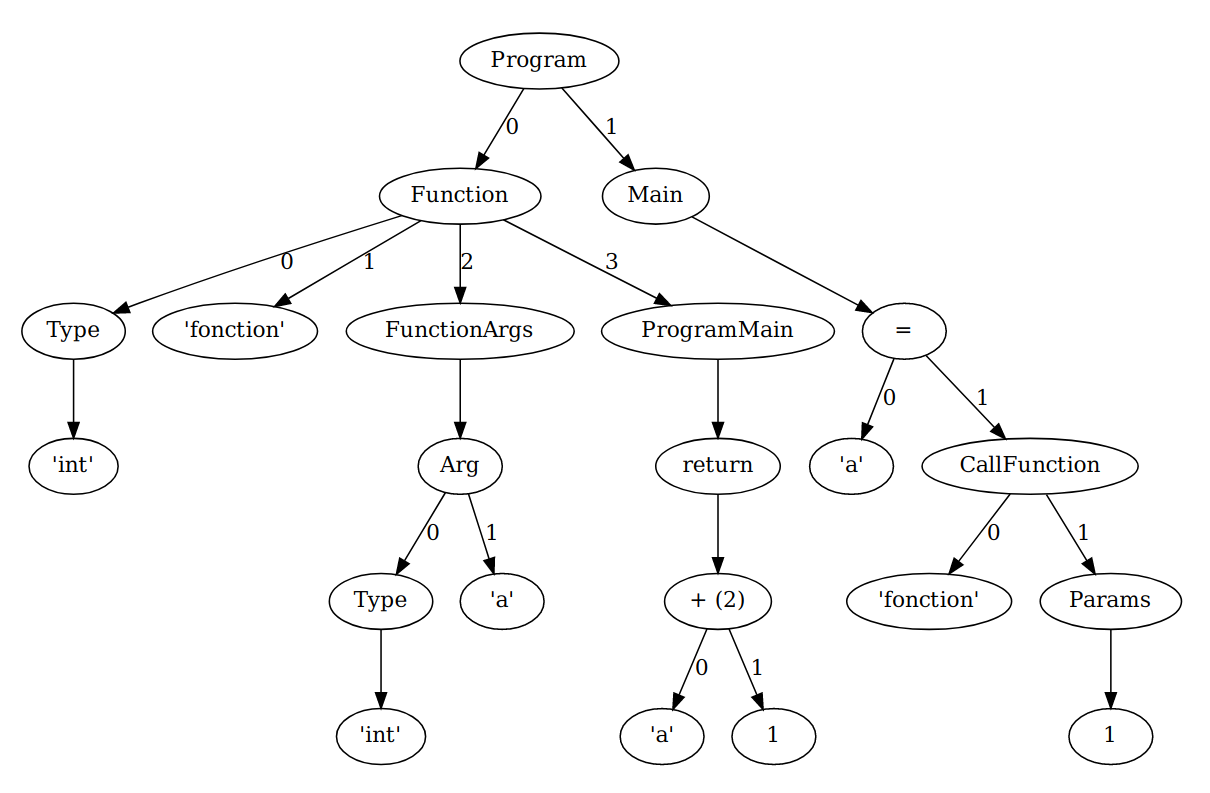
\includegraphics[width=0.8\textwidth]{./images/exemple_ast_fonction.png}
    \caption{Exemple AST fonction}\label{exemple_fonction}
\end{figure}

\section{Gestion des indentations}

La gestion des indentations dans notre programme permet de détecter les indentations et dédentations en python et les remplacer par des \textbf{\{\}} en \textbf{C++}
ainsi que gérer la portée.

\subsection*{Analyse lexicale}

Lors de l'analyse lexicale, les indentations sont détectées par un regex puis ajoutées dans un stack avec sa valeur d'indentation.
Cette valeur d'indentation visa à identifier le niveau de profondeur de l'indentation.

Après avoir détecté l'indentation et sa valeur, le token doit être modifié pour devenir une nouvelle ligne si le niveau de profondeur est le même.
Et dans le cas où le niveau de profondeur est plus bas que l'indentation précédente, le token devient une dédentation.
\newline
\newline
Sur le code ci-dessous, un exemple de l'évolution de la valeur d'indentation:
\lstset{language=Python}
\begin{lstlisting}
def fo(x):  # INDENT value = 0
    if x > 5:   # INDENT value = 1
        print("bigger than 5")  # INDENT value = 2
        print("it's great!")    # NEWLINE
fo(6)   # DEDENT value = 2
\end{lstlisting}

\subsection*{Analyse syntaxique}

À la fin de l'analyse lexicale, les tokens d'indentations et dédentations contiennent leurs valeurs respectives.
Cependant pour grandement simplifier l'analyse syntaxique avant de passer les tokens dans le parseur, les tokens de dédentations sont multipliés par leur valeur.
Par exemple pour un token «DEDENT(2)» on renvoie 2 fois le token «DEDENT».
Cela permet d'avoir des blocs bien définis commençant par «INDENT» et finissant par «DEDENT»

\section{Gestion des erreurs}

Lors de la transpilation nous détectons différents types d'erreurs sur le code.
\newline
\begin{itemize}
    \item Contrôle de type sur le passage de paramètre dans une fonction
    \item Contrôle de type sur le type de retour d'une fonction
    \item Contrôle d'existence des variables globales
    \item Division par zéro
\end{itemize}

\chapter{Tests et résultats}

Ce programme a été testé avec plusieurs scripts python se trouvant dans le dossier \textbf{src/test}.
Sur les figures \ref{exemple_python} et \ref{exemple_cpp} vous trouverez un exemple de code python transformé en code C++.
Ainsi que l'arbre syntaxique généré par le parseur à la figure \ref{exemple_ast}.

\begin{figure}[h]
    \centering
    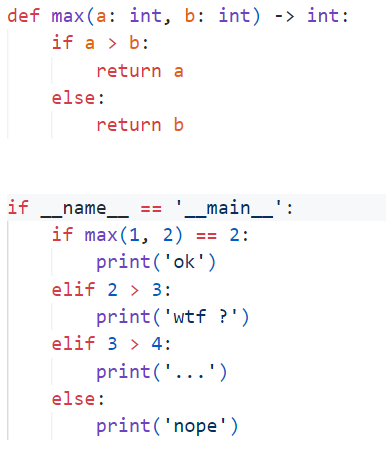
\includegraphics[width=0.4\textwidth]{./images/exemple_python.png}
    \caption{Exemple code python}\label{exemple_python}
\end{figure}

\begin{figure}[h]
    \centering
    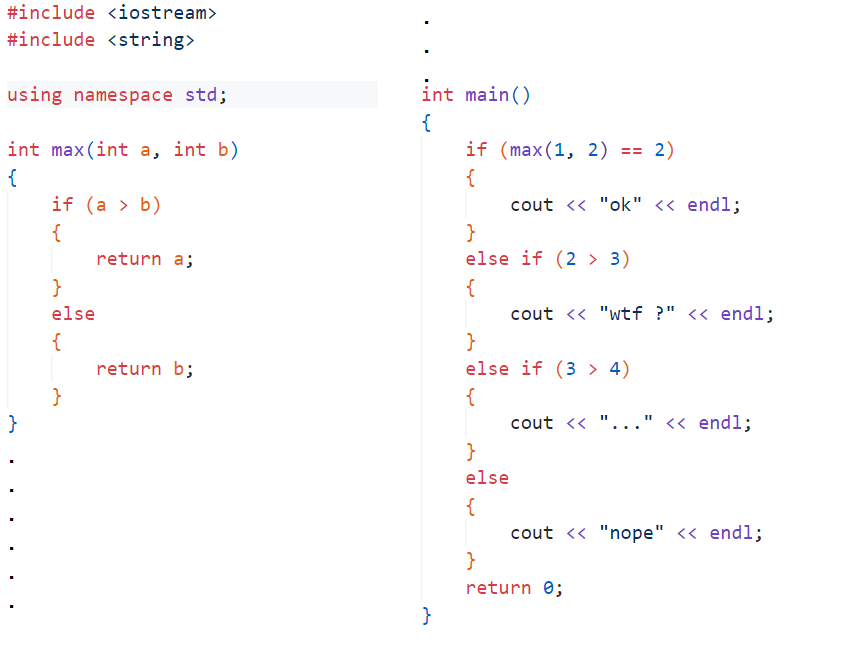
\includegraphics[width=0.8\textwidth]{./images/exemple_cpp.png}
    \caption{Exemple code C++}\label{exemple_cpp}
\end{figure}

\begin{figure}[h]
    \centering
    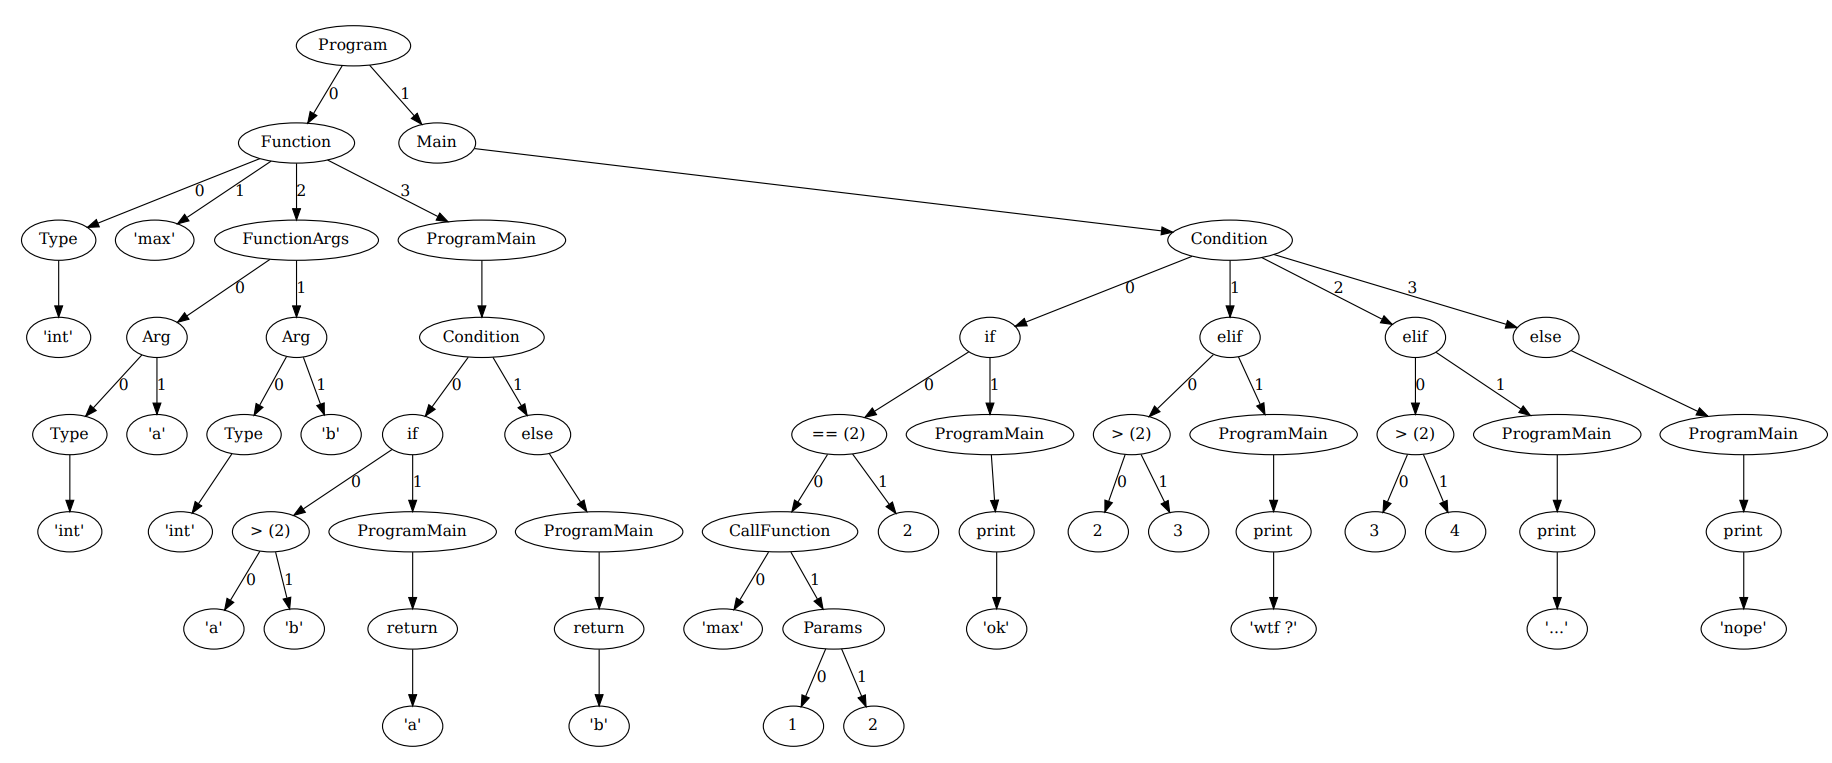
\includegraphics[width=1\textwidth]{./images/exemple_ast.png}
    \caption{Exemple AST}\label{exemple_ast}
\end{figure}

\chapter{Conclusion}

Sur la base des résultats obtenus, notre programme est capable de transcrire du python en \textbf{C++} avec certaines restrictions.
Notamment, le typage des fonctions et le code sont obligés d'avoir une  fonction \textbf{main} pour que le transpilateur fonctionne.
Le programme est également capable de produire des warnings ainsi que des messages d'erreurs.

\chapter*{Annexe}

~\label{annexe:grammar}
\begin{verbatim}
Rule 0     S' -> programs
Rule 1     programs -> program main
Rule 2     programs -> main
Rule 3     main -> MAIN INDENT program_main DEDENT
Rule 4     program -> statement
Rule 5     program -> statement NEWLINE
Rule 6     program -> program statement NEWLINE
Rule 7     program -> program statement
Rule 8     statement -> assignation
Rule 9     statement -> function
Rule 10    function -> DEF ID ( args ) ARROW TYPE : INDENT program_main DEDENT
Rule 11    function -> DEF ID ( ) ARROW TYPE : INDENT program_main DEDENT
Rule 12    args -> arg
Rule 13    args -> args , arg
Rule 14    arg -> ID : TYPE
Rule 15    program_main -> statement_main NEWLINE
Rule 16    program_main -> statement_main
Rule 17    program_main -> program_main statement_main NEWLINE
Rule 18    program_main -> program_main statement_main
Rule 19    statement_main -> assignation
Rule 20    statement_main -> global
Rule 21    statement_main -> structure_main
Rule 22    statement_main -> return_func
Rule 23    statement_main -> call_func
Rule 24    statement_main -> condition
Rule 25    global -> GLOBAL ID
Rule 26    statement_main -> PRINT expression
Rule 27    return_func -> RETURN expression
Rule 28    assignation -> ID = expression
Rule 29    structure_main -> WHILE expression : INDENT program_main DEDENT
Rule 30    condition -> if_stmt
Rule 31    condition -> if_stmt else_stmt
Rule 32    condition -> if_stmt elifs else_stmt
Rule 33    if_stmt -> IF expression : INDENT program_main DEDENT
Rule 34    else_stmt -> ELSE : INDENT program_main DEDENT
Rule 35    elifs -> elif_stmt
Rule 36    elifs -> elifs elif_stmt
Rule 37    elif_stmt -> ELIF expression : INDENT program_main DEDENT
Rule 38    expression -> call_func
Rule 39    call_func -> ID ( )
Rule 40    call_func -> ID ( list_expr )
Rule 41    list_expr -> expression
Rule 42    list_expr -> list_expr , expression
Rule 43    expression -> NUMBER
Rule 44    expression -> ID
Rule 45    expression -> TEXT
Rule 46    expression -> BOOL
Rule 47    expression -> ( expression )
Rule 48    expression -> expression + expression
Rule 49    expression -> expression - expression
Rule 50    expression -> expression * expression
Rule 51    expression -> expression / expression
Rule 52    expression -> expression % expression
Rule 53    expression -> + expression
Rule 54    expression -> - expression
Rule 55    expression -> expression AND expression
Rule 56    expression -> expression OR expression
Rule 57    expression -> expression EQ expression
Rule 58    expression -> expression NE expression
Rule 59    expression -> expression GE expression
Rule 60    expression -> expression LE expression
Rule 61    expression -> expression > expression
Rule 62    expression -> expression < expression
Rule 63    expression -> NOT expression
Rule 64    NUMBER -> INT
Rule 65    NUMBER -> FLOAT
Rule 66    TEXT -> STRING
Rule 67    TEXT -> CHAR
Rule 68    BOOL -> TRUE
Rule 69    BOOL -> FALSE
\end{verbatim}